\chapter{Human 3D pose from depth images}
%% WHAT IS IMPLEMETED
%% WHY DOES IT REPRESENT A PROGRESS IN RESEARCH

To train any network using supervised learning, we need large amounts of training data. One of the goals for the MECS project is to do \emph{Human Activity Recognition (HAR)}, so one can track the user from day to day and look for patterns that could lead to worsening living conditions. We also want to be able to recognize the activity from any viewpoint, and this is where a 2D approach will lack robustness. This is because any HAR model trained solely on 2D data, will only be able to recognize the activity from the views it has seen the activity being preformed. A 3D approach will provide us with robustness in respect to view-independentness.

We implemented an algorithm for extraction of human pose in 3D.
Applying methods used on 3-channel (RGB) images to depth images, we show that the same methods can be used to extract objects in 2d images, can be used to extract objects in depth images as well, when it comes to human pose.

As in \cite{cao2017realtime} we will use two networks to create the \gls{paf}s and the confidence maps for the joints. However, instead of training on 3-channel RGB images, we will use a single channel depth image to discover the body landmarks/joints.
However, since depth images are single channel, and thus have less information than the RGB images, we propose using a shallower network. This also means we have to do the first step of feature extraction which was already done in a
However since the depth images are less detailed than normal RGB images some landmarks might be harder to detect, such as eyes or nose or placing the joint on outstreched limbs.


This was considered when preparing the training data.

\section{Architecture}

When we are creating a neural network, it is often helpful to have in mind \emph{what} we want to detect in each layer. It is therefore segregated into a couple of different steps to make it easier to follow along.

The architecture of this project is \emph{recurrent} in that it repeats itself for a number of iterations. As with the \cite{cao2017realtime} architecture, we have to have a first step which produces the first ouptuts we can use in later steps. However, this step is not illustrated in Fig.\ref{fig:arch_main}, since the first step will be identical to the next steps except it won't have the additional inputs produced by the outputs of the previous step.

\begin{figure}[h]
  \centering
  \includegraphics[width=\textwidth]{img/architecture_main}
  \caption[Main architecture]{Main architecture. \gls{cnn}s are illustrated as hourglass networks, but this is not neccessarily representative of the final architecture. A depth image is fed to a depth-feature extraction network (\ref{subsec:depth_feature}) which in consecutive steps are combined with output \gls{paf}s and joint confidence maps, before this is fed to the 3D object detection networks (\ref{subsec:obj_detect}). These are run for a small number of iterations to get some estimate for the \gls{paf}s and confidence maps, before we move on to the assembly step. For each of the skeletons detected (with a ceiling for maximum detected skeletons) the skeletons with the strongest evidence are assembled. In the case that a body landmark is not found, we use preconcieved coordinates from a standard defined skeleton. The coordinate frame of the skeleton in the articulation step till be the root joint (middle hip) with the z-axis pointing up, and the y-axis orthogonal to the line through the two side hip joints. The articulation network (\ref{subsec:articulation}) tries to scale and articulate the skeleton based on detected evidences. In the disassembly step, we place all the skeletons back into the camera coordinate frames, and update the \gls{paf}s and confidence maps with confidences and placements from the articulation network, and use them in the following steps. This is repeated a small number of times (3-4).}
  \label{fig:arch_main}
\end{figure}

\subsection{Depth feature extraction}\label{subsec:depth_feature}
For each pixel in the current layer of the \ref{cnn}, we collect information from a filter-sized portion of the previous layer. This means that deeper layers look at a larger and larger portion of the input layer. This is useful for detecting connections between large-scale structures. This also means that after a certain depth, there may not be any more useful information.

In our experiments we'll try different depths for feature extraction.

Some of these features might be desirable as inputs for later layers in object classification.

This network is built from the ground up. Therefore we want some layers to for example detect edges, and one for detecting slanting gradients, or connected surfaces. For limbs, we might want to find surfaces that are shaped like tubes or oblong spheroids.

\subsection{3D object detection}\label{subsec:obj_detect}
In this part of the network we borrow some of the architecture described in \cite{cao2017realtime}. The purpose is to find joints and limbs and put them into \gls{paf}s or joint confidence maps. 

\subsection{Articulation network}\label{subsec:articulation}
Input: Coordinates and confidences for each joint (if not detected, confidence is 0) and the mean \gls{paf} vector for each limb.
Here, we get some coordinates for different joints, along with the confidences for those coordinates. The network will try to find out what it thinks the joints with low confidences, or no detections, should be. It is hypotesized that this network will learn things like symmetry (left and right limbs should have the same length), proportionality (limbs should be proportional to each other), possible articulations and natural poses.

For joints which we haven't detected or have very low confidence for, the network will input some standard coordinates for that joint, scaled by the limbs we already have the strongest confidences for. The standard scaling/coordinates is hard-coded, based on the human anatomy surveys in \cite{bodySegmentParams}. The exception is eyes and ears, which is set to a best guess. In addition, the depth coordinate for each joint is set to 0. Numbering and a visualization of the skeleton can be seen in Figure \ref{fig:skeleton_markers}.

The architecture is visualized as a simple fully connected neural network. Though, it might be enough to connect the neurons responsible for connected limbs. A neuron in the second layer connected to the foot, knee and one of the hip-joints does not need to be connected to the inputs from a hand or shoulder. Subsequent hidden layers can however be fully connected.

If we had some input describing the direction of the camera, and the \gls{visual_hull} containing the undetected points, this network may preform better. However, that would require a fundamental change to the network, which is not done in this work.

This network will also be trained separatley, as all it needs is poses and random confidences as inputs.


\section{Training data preparation}

Skeleton models
\begin{figure}[h]

  \begin{floatrow}
    \ffigbox{
      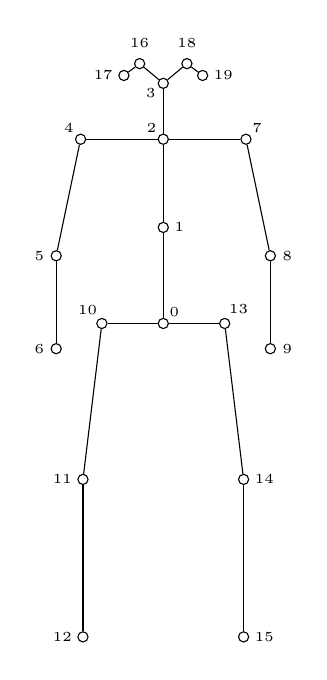
\begin{tikzpicture}[
          every node/.style={draw,circle,minimum size=.06cm, inner sep=1.3pt}
        ]
        \tiny
        %% \draw[help lines, step=5mm, gray!20] (-4,-4) grid (3,4);
        %% Standard coordinates => (orig.coords) - (0, .2)
        \node[label={[label distance=-.2mm]200:{3}}] (nose) at (0,3.25) {};
        \node[label={[label distance=-.2mm]140:{2}}] (neck) at (0,2.54) {};
        \node[label={[label distance=-.2mm]0:{1}}] (back) at (0,1.42) {};
        
        \node[label={[label distance=-.1mm]90:{16}}] (reye) at (-.3,3.5) {};
        \node[label={[label distance=-.1mm]90:{18}}] (leye) at (.3,3.5) {};

        \node[label={[label distance=-.1mm]180:{17}}] (rear) at (-.5,3.35) {};
        \node[label={[label distance=-.1mm]0:{19}}] (lear) at (.5,3.35) {};

        \node[label={[label distance=-.2mm]140:{4}}] (rshoulder) at (-1.05,2.54) {};
        \node[label={[label distance=-.2mm]50:{7}}] (lshoulder) at (1.05,2.54) {};
        
        \node[label={[label distance=-.1mm]180:{5}}] (relbow) at (-1.36,1.06) {};
        \node[label={[label distance=-.1mm]0:{8}}] (lelbow) at (1.36,1.06) {};

        \node[label={[label distance=-.1mm]180:{6}}] (rwrist) at (-1.36,-.12) {};
        \node[label={[label distance=-.1mm]0:{9}}] (lwrist) at (1.36,-.12) {};

        \node[label={[label distance=-.2mm]140:{10}}] (rhip) at (-.78,.2) {};
        \node[label={[label distance=-.2mm]50:{13}}] (lhip) at (.78,.2) {};
        \node[label={[label distance=-.2mm]50:{0}}] (mhip) at (0, .2) {};

        \node[label={[label distance=-.1mm]180:{11}}] (rknee) at (-1.02,-1.78) {};
        \node[label={[label distance=-.1mm]0:{14}}] (lknee) at (1.02,-1.78) {};

        \node[label={[label distance=-.1mm]180:{12}}] (rankle) at (-1.02,-3.78) {};
        \node[label={[label distance=-.1mm]0:{15}}] (lankle) at (1.02,-3.78) {};

        %% \draw[blue] (0,0) circle [radius=.06cm];

        \draw (nose) -- (neck);
        \draw (neck) -- (back);
        \draw (back) -- (mhip);
        \draw (reye) -- (nose); \draw (leye) -- (nose);
        \draw (reye) -- (rear); \draw (leye) -- (lear);
        
        \draw (neck) -- (rshoulder); \draw (neck) -- (lshoulder);
        %% \draw (neck) -- (rhip); \draw (neck) -- (lhip);
        \draw (mhip) -- (rhip); \draw (mhip) -- (lhip);

        \draw (rshoulder) -- (relbow); \draw (lshoulder) -- (lelbow);
        \draw (rwrist) -- (relbow); \draw (lwrist) -- (lelbow);

        \draw (rhip) -- (rknee); \draw (lhip) -- (lknee);
        \draw (rknee) -- (rankle); \draw (lknee) -- (lankle);
      \end{tikzpicture}
    }
    {
      \caption[Numbering for keypoint markers]{Numbering for detected landmarks/keypoint markers.}
      \label{fig:skeleton_markers}
    }
    %% \end{figure}
    %% \begin{table}
    \capbtabbox{
      \footnotesize
      \begin{tabular}[H]{|r l r|}
        \hline
        ID & Description & Std.Coord. \\ \hline
        0  & Middle hip & (0.00, 0.00) \\
        1  & Middle back & (0.00, 1.22) \\
        2  & Neck & (0.00, 2.34) \\
        3  & Nose & (0.00, 3.05) \\
        4  & Right shoulder & (-1.05, 2.34) \\
        5  & Right elbow & (-1.36, 0.86) \\
        6  & Right wrist & (-1.36, -0.32) \\
        7  & Left shoulder & (1.05, 2.34) \\
        8  & Left elbow & (1.36, 0.86) \\
        9  & Left wrist & (1.36, -0.32) \\
        10 & Right hip & (-0.78, 0.00) \\
        11 & Right knee & (-1.02, -1.98) \\
        12 & Right ankle & (-1.02, -3.98) \\
        13 & Left hip & (0.78, 0.00) \\
        14 & Left knee & (1.02, -1.98) \\
        15 & Left ankle & (1.02, -3.98) \\
        16 & Right eye & (-0.30, 3.30) \\
        17 & Right ear & (-0.50, 3.15) \\
        18 & Left eye & (0.30, 3.30) \\
        19 & Left ear & (0.50, 3.15) \\
        \hline
      \end{tabular}
    }{
      \caption[Names/coordinates for detected landmarks]{Numberings, names/descriptions and standard coordinates for recognized landmarks}
      \label{tab:openpose_body_ids}
    }
  \end{floatrow}          
\end{figure}

%% \section{2D detection transfer}

%% (First ideas.)

%% Torso placement and tree structure for placing.

%% Fit to human standard model (rules for symmetry and lengths)

%% Occlusion problem, and interpolated points, visual hull constraints

%% We train the network on both depth images and a kinematic model of each 3D ground truth location.

%% \section{Pose from CNN over depth maps}

%% We create a separate 'side-view' detection map for each 'frontal' detection map. This reduces the convolution operations, since we don't have to convolve over the whole 3D space.
